\section{Auswertung}
\subsection{Die Drillachse}
\subsubsection{Die Winkelrichtgröße}
Um die Winkelrichtgröße $D$ der Drillachse zu bestimmen wird Gleichung
%\eqref{eq:??}
verwendet. Die benötigten werte für die Kraft $F$, den Radius $r$ und den Winkel $\phi$ lassen sich der Tabelle %\ref{tab:tab1}
entnehmen.
\[D=\SI{0,0256(6)}{\joule}\]
\begin{table}
	\centering
	\caption{Messdaten zur Winkelrichtgrößenbestimmung}
	\sisetup{table-format=1.2}
	\begin{tabular}{S[table-format=3.2] S[table-format=3.2]S[table-format=3.2]S[table-format=3.2]}
		\toprule
		{$F/\si[per-mode=reciprocal]{\newton}$}&{$r/\si[per-mode=reciprocal]{\metre}$}&{$\phi/\si[per-mode=reciprocal]{\radian}$} \\
		\midrule
		0,12 & 0,119 & 0,524 \\
		0,19 & 0,119 & 0,873 \\		
		0,38 & 0,059 & 0,873 \\
		0,16 & 0,190 & 1,047 \\
		0,20 & 0,170 & 1,222 \\
		0,30 & 0,110 & 1,396 \\
		0,28 & 0,139 & 1,571 \\	
		0,27 & 0,159 & 1,745 \\
		0,30 & 0,170 & 2,094 \\
		0,22 & 0,239 & 2,269 \\
		\bottomrule
	\end{tabular}
	%\label{tab:tab1}
\end{table}
\subsubsection{Eigendrehmoment}
Zur Bestimmung des Eigendrehmoments werden zwei Zylinder mit dem Durchmesser $d = \SI{0,035}{\metre}$, der Höhe $h = \SI{0,03}{\metre}$ und der Masse $m = \SI{0,2218}{\kilogram}$ benutzt.\newline Die Verbindungsstange wird als masselos angenommen und wird daher nicht berücksichtigt.
\begin{figure}
\centering
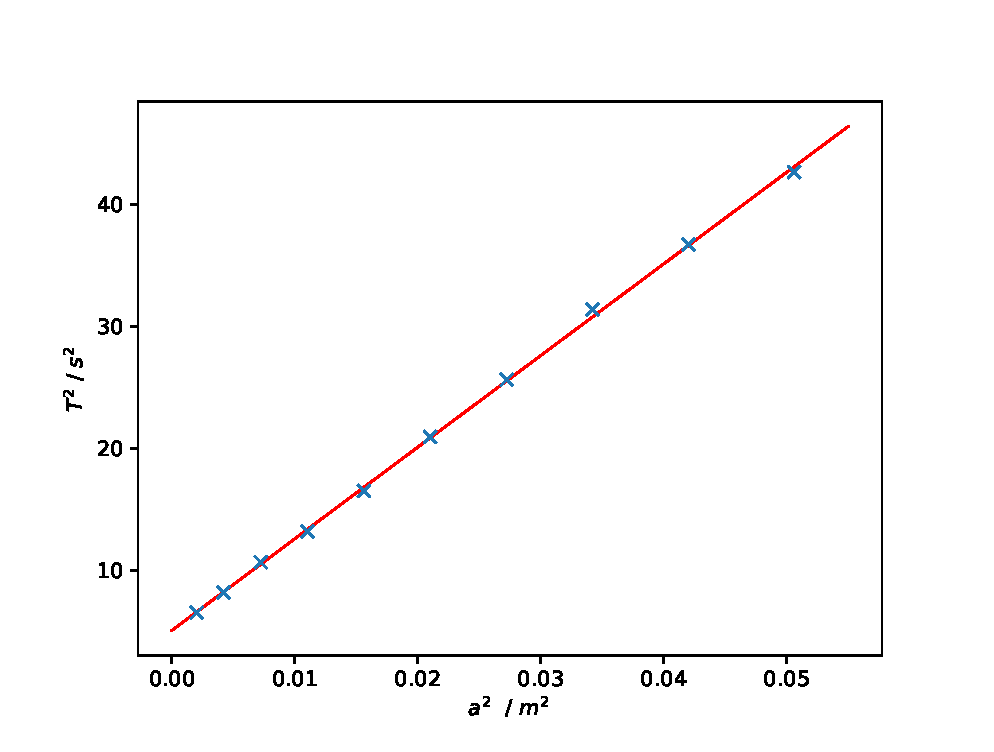
\includegraphics[scale = .75,keepaspectratio]
	{content/images/plot1.eps}
\caption{Graph der Messdaten zur Bestimmung des Eigendrehmoments der Drillachse}%\label{fig:abb1}
\end{figure}
\begin{table}
	\centering
	\caption{Messdaten zur Eigendrehmomentbestimmung}
	\sisetup{table-format=1.2}
	\begin{tabular}{S[table-format=3.2] S[table-format=3.2]S[table-format=3.2]S[table-format=3.2]}
		\toprule
		{$r/\si[per-mode=reciprocal]{\metre}$}&{$T/\si[per-mode=reciprocal]{\second}$} \\
		\midrule
		0,045 & 2,5525 \\
		0,065 & 2,86 \\
		0,085 & 3,2675 \\
		0,105 & 3,63 \\
		0,125 & 4,065 \\
		0,145 & 4,575 \\
		0,165 & 5,06 \\
		0,185 & 5,6 \\
		0,205 & 6,06 \\
		0,225 & 6,53 \\
		\bottomrule
	\end{tabular}
	%\label{tab:tab2}
\end{table}
Die Werte für das Quadrat der Periodendauer $T$ und des Abstands $a$ aus Tabelle %\ref{tab:tab2}
sind im Graph %\ref{fig:abb1}
gegeneinander aufgetragen.
Mit Gleichung %\eqref{eq:??}
ergibt sich für das Drehmoment $I_.D$ der Drillachse:
\[I_.D=\SI{0,01026(4)}{\kilogram\metre\squared}\]
\subsection{Das Drehmoment einer Kugel}
